% To je predloga za poročila o domačih nalogah pri predmetih, katerih
% nosilec je Blaž Zupan. Seveda lahko tudi dodaš kakšen nov, zanimiv
% in uporaben element, ki ga v tej predlogi (še) ni. Več o LaTeX-u izveš na
% spletu, na primer na http://tobi.oetiker.ch/lshort/lshort.pdf.
%
% To predlogo lahko spremeniš v PDF dokument s pomočjo programa
% pdflatex, ki je del standardne instalacije LaTeX programov.

\documentclass[a4paper,11pt]{article}
\usepackage{a4wide}
\usepackage{fullpage}
\usepackage[utf8x]{inputenc}
\usepackage[slovene]{babel}
\selectlanguage{slovene}
\usepackage[toc,page]{appendix}
\usepackage[pdftex]{graphicx} % za slike
\usepackage{setspace}
\usepackage{color}
\definecolor{light-gray}{gray}{0.95}
\usepackage{listings} % za vključevanje kode
\usepackage{hyperref}
\usepackage[]{algorithm2e}
\usepackage{program}
\usepackage{algpseudocode}
\renewcommand{\baselinestretch}{1.2} % za boljšo berljivost večji razmak
\renewcommand{\appendixpagename}{Priloge}

\lstset{ % nastavitve za izpis kode, sem lahko tudi kaj dodaš/spremeniš
language=Python,
basicstyle=\footnotesize,
basicstyle=\ttfamily\footnotesize\setstretch{1},
backgroundcolor=\color{light-gray},
}

\title{Modeliranje časovnih trendov z markovskimi verigami \\ \large  Poročilo izvorne kode (serijski algoritem)}
\author{Jaka Kordež \\ Anže Gregorc}
\date{\today}

\begin{document}

\maketitle

\section{Uvod}

Pri predmetu bomo spoznavali sisteme za vzporedno in porazdeljeno procesiranje. Izbrali smo problem, ki ga bomo v skupinah po dva tekom semestra nadgrajevali s pomočjo različnih pristopov za paralelno programiranje. Tokrat pa je poročilo namenjeno serijskem algoritmu, ki še ni paraleliziran. 

\section{Opis problema}

Naš namen je v bližnji prihodnosti predvideti ceno določenega trga s pomočjo markovskih verig. Te si zapomnijo le zadnje stanje problema, za to ne pričakujeva prav zelo dobrih rezultatov. Stanje sva definirala kot zaporedje zadnjih 8 vrednosti premikov cen. Vendar je primerna za paralelizacijo, saj je glavni element markovskih verig matrika.

\section{Podatki}

Našla sva podatke valutnega para EUR/USD iz spletne strani \url{http://www.histdata.com/download-free-forex-historical-data/?/metatrader/1-minute-bar-quotes/EURUSD}. Skupno je 8723490 minutnih podatkov o ceni, uporabila sva ceno ob koncu (ang. close price). Podatki so urejeni v csv datoteki tako: (čas v unix formatu),cena. Primer vrstice: 959704020,0.930200 pomeni 30. maj 2000 ob 16:27 GMT je bila cena 0.930200 EUR za 1 USD.

\section{Metode}

Program deluje tako, da pri branju podatkov shrani razliko v ceni med zaporednima cenama trga. Nato te cene pretvori v stanja, ki se jih uporablja v markovskih verigah. Meja med stanji je lahko določena eksponentno. Na primer: če imamo 6 stanj bodo meje med stanji za določeno razliko postavljene na -0.01; -0.0025; 0.0; 0.0025; 0.01. Ceno je torej možno pretvoriti na več načinov. Trenutno je namen implementirati dva načina. Drugi način pa je: če zaporedje cene nekaj časa konstantno narašča oziroma pada, se razliko pomnoži še s prejšnjim stanjem. Tukaj je možna še kakšna sprememba, če bi kakšen drug način pretvorbe vrnil boljše rezultate. Stanja se potem vnašajo v markovsko verigo. S pomočjo drsečega okna se zadnjih 5 zaporednih podatkov pretvori v indeks stolpca matrike in prištejemo 1 v vrstico trenutnega stanja. Nato se matriko normaliriza  po vrsticah, da dobimo pravo markovsko verigo. Možen dodatek matriki pa je povprečiti rezultate napovedi, ki predstavljajo dvig cene ter posebej spust cene. Tako lažje interpretiramo matriko, saj potem pove verjetnost padca oziroma rasti cene, če poznamo zadnjih 8 zaporednih vrednosti valute.

\subsection{Psevdokoda}

\begin{program}
\mbox{Osnovni algoritem za kreiranje matrike}
\BEGIN \\
 data := read(filename)\; 
 states := convert To States(data)\; 
 matrix := create matrix()\; 
\FOR i:=0 \TO data.length \STEP 1 \DO
     index := toIndex(states); \\
  matrix[index] := matrix[index] + 1\; \OD %

 normalize(matrix)\;
\END
\end{program}

\subsection{Glavne podatkovne strukture}
\textbf{Vektor stanj:} tabela časovno zaporednih stanj trga \\
\textbf{Markovska matrika: } matrika, ki pokaže porazdelitev verjetnosti naslednjega stanja, če poznamo trenutno stanje


\section{Rezultati}

Z markovsko verigo se je možno sprehajati po naslednjih stanjih in tako rekoč napovedati ceno časovno zelo daleč naprej, vendar pa to prav zagotovo ne bodo več smiselni podatki. Ta naloga je bolj usmerjena napovedovanju dviga cene le v naslednjem koraku. 

\(
9 -> 0 -> 9 -> 5 -> 9 -> 0 -> 2 -> 1 -> -0.962963 \\
9 -> 0 -> 9 -> 0 -> 9 -> 7 -> 3 -> 0 -> 0.971429 \\
1 -> 9 -> 1 -> 0 -> 9 -> 0 -> 8 -> 1 -> -0.960000 \\
9 -> 0 -> 8 -> 9 -> 1 -> 0 -> 1 -> 1 -> -0.961538 \\
9 -> 8 -> 9 -> 8 -> 9 -> 0 -> 3 -> 0 -> 0.888889 \\
8 -> 9 -> 0 -> 1 -> 9 -> 1 -> 9 -> 1 -> -0.960000 \\
9 -> 0 -> 1 -> 0 -> 8 -> 9 -> 8 -> 1 -> -0.962963 \\
9 -> 0 -> 9 -> 0 -> 9 -> 0 -> 9 -> 1 -> -0.968690 \\
0 -> 9 -> 5 -> 9 -> 0 -> 9 -> 7 -> 1 -> -0.964286 \\
0 -> 9 -> 7 -> 9 -> 0 -> 9 -> 2 -> 1 -> -0.966667 \\
\)
\\
Zgornji podatki povedo, da v primeru takih zaporedij stanj razlik v ceni (cela števila predstavljajo stanja) je verjetnost (ki je zadnje, decimalno število), da bo cena narastla. Te podatki so zanimivi, saj imajo visoko verjetnost napovedi trenda valute v naslednjem koraku. Minus pred verjetnostjo pomeni, da je taka verjetnost, da bo cena padla. Meje med stanjem v danem primeru:  -0.000033, -0.000011 -0.000004, -0.000001, 0.000000, 0.000001, 0.000004, 0.000011, 0.000033. Stanje 0 je pod prvo mejo (-0.000033), stanje 1 med prvo in drugo in tako naprej.

\subsection{Časovna zahtevnost}
Algoritem je odvisen od dveh stvari: velikosti podatkov in številom stanj. Ker imamo samo en sklop podatkov lahko pri časovni zahtevnosti zanemarimo, drugače pa bi bila O(n), pri čemer je n število podatkov. Število stanj pa lahko spreminjamo in ker se matrika povečuje eksponentno, ko število stanj povečujemo linearno. torej \(  O(s^8) \) kjer je s število stanj in 8 ker je predhodno stanje sestavljeno iz zaporedja zadnjih osmih rezlik v ceni. Graf dejanskega časovnega izvajanja v odvisnosti od števila stanj lepo pokaže polinomsko naraščanje, torej se sklada s teoretično oceno.

\begin{figure}[htbp]
\begin{center}
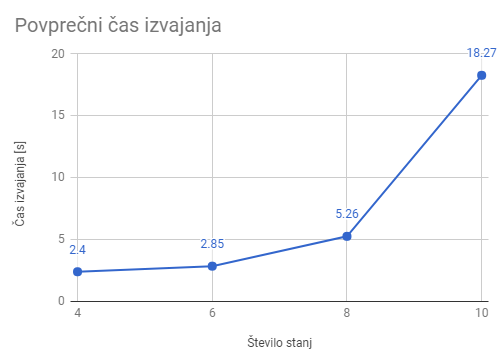
\includegraphics[scale=0.8]{graf1.png}
\label{graf}
\end{center}
\end{figure}

\begin{figure}[htbp]
\begin{center}
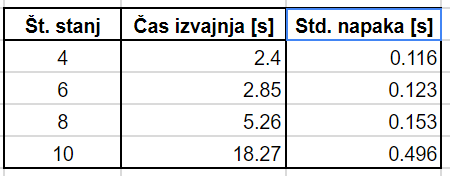
\includegraphics[scale=0.8]{tabela1.png}
\label{graf}
\caption{Tabela prikazuje časovno zahtevnost in standardno deviacijo v odvisnosti od števila stanj}
\end{center}
\end{figure}




\end{document}
